\documentclass[12pt,letterpaper]{exam}
\usepackage[lmargin=1in,rmargin=1in,tmargin=1in,bmargin=1in]{geometry}
\usepackage{../style/exams}

% -------------------
% Course & Exam Information
% -------------------
\newcommand{\course}{MAT 108: Exam 3}
\renewcommand{\term}{Spring -- 2023}
\newcommand{\examdate}{05/03/2023}
\newcommand{\timelimit}{85 Minutes}

\setbool{hideans}{true} % Student: True; Instructor: False

% -------------------
% Content
% -------------------
\begin{document}

\examtitle
\instructions{Write your name on the appropriate line on the exam cover sheet. This exam contains \numpages\ pages (including this cover page) and \numquestions\ questions. Check that you have every page of the exam. Answer the questions in the spaces provided on the question sheets. Be sure to answer every part of each question and show all your work. If you run out of room for an answer, continue on the back of the page --- being sure to indicate the problem number.} 
\scores
\bottomline
\newpage

% ---------
% Questions
% ---------
\begin{questions}

% Question 1
\newpage
\question[10] Define the following vectors:
	\[
	\mathbf{u}= \begin{pmatrix} 3 \\ -2 \\ 0 \end{pmatrix} \qquad 
	\mathbf{v}= \begin{pmatrix} -4 \\ 1 \\ 5 \end{pmatrix}
	\]
Showing all your work, compute the following:
	\begin{enumerate}[(a)]
	\item $-2 \mathbf{v}$
	\item $\mathbf{v} - 3 \mathbf{u}$
	\item $\mathbf{u} \cdot \mathbf{v}$
	\end{enumerate}



% Question 2
\newpage
\question[10] Define the following matrices:
	\[
	A= \begin{pmatrix} 1 & 0 & 3 \\ 2 & -1 & 4 \\ 0 & 6 & -2 \end{pmatrix} \qquad
	B= \begin{pmatrix} 1 & 8 \\ -2 & 0 \\ 0 & 3 \\ 9 & -6 \end{pmatrix} \qquad
	C= \begin{pmatrix} 2 & -7 & -9 \\ 3 & 6 & 5 \\ 8 & -2 & -3 \end{pmatrix}
	\]

\begin{enumerate}[(a)]
\item Compute $B^T$. 
\item Showing all your work, compute $-2C$.
\item Showing all your work, compute $C - A$. 
\item Explain why one cannot form the product $AB$. 
\end{enumerate}



% Question 3
\newpage
\question[10] Consider the system of linear equations shown below:
	\[
	\begin{aligned}
	2x + 3y&= 1 \\
	4x + 5y&= 5
	\end{aligned}
	\]
Let $A$ be the coefficient matrix and $\mathbf{b}$ be the constant vector associated to the system of equations above. 
        \begin{enumerate}[(a)]
        \item Write the system of equations above in the form $A\mathbf{x}= \mathbf{b}$. 
        \item Explain why $A^{-1}$ exists and find $A^{-1}$. 
        \item Use $A^{-1}$ to find the solution to the system of equations above. 
        \end{enumerate}



% Question 4
\newpage
\question[10] The matrix below is the initial augmented matrix coming from a system of linear equations. Find the original system of equations. 
	\[
	\begin{pmatrix} 3 & -1 & 5 & 2 & 8 \\ 7 & 0 & 2 & 8 & -11 \\ 4 & 1 & -1 & 6 & 15 \end{pmatrix}
	\]



% Question 5
\newpage
\question[10] The matrix shown below is the RREF of an augmented matrix coming from a system of linear equations. Does the corresponding system of equations have a solution? If so, find the solution(s). If not, explain why. 
	\[
	\begin{pmatrix}
	1 & 0 & 0 & 0 & 4 \\
	0 & 1 & 0 & 0 & 0 \\
	0 & 0 & 1 & 0 & -5 \\
	0 & 0 & 0 & 1 & 3
	\end{pmatrix}
	\]



% Question 6
\newpage
\question[10] The matrix shown below is the REF of an augmented matrix coming from a system of linear equations. Does the corresponding system of equations have a solution? If so, find the solution(s). If not, explain why. 
	\[
	\begin{pmatrix}
	1 & 0 & 0 & -1 \\
	0 & 1 & 0 & 9 \\
	0 & 0 & 1 & 2 \\
	0 & 0 & 0 & 1
	\end{pmatrix}
	\]



% Question 7
\newpage
\question[10] The matrix shown below is the RREF of an augmented matrix coming from a system of linear equations. Does the corresponding system of equations have a solution? If so, find the solution(s). If not, explain why. 
	\[
	\begin{pmatrix}
	1 & 2 & 0 & 5 \\
	0 & 0 & 1 & 4 \\
	0 & 0 & 0 & 0 
	\end{pmatrix}
	\]



% Question 8
\newpage
\question[10] Consider the function $f(x_1, x_2)= 3x_1 - x_2$ on the region shown below. \par
	\[
	\fbox{
	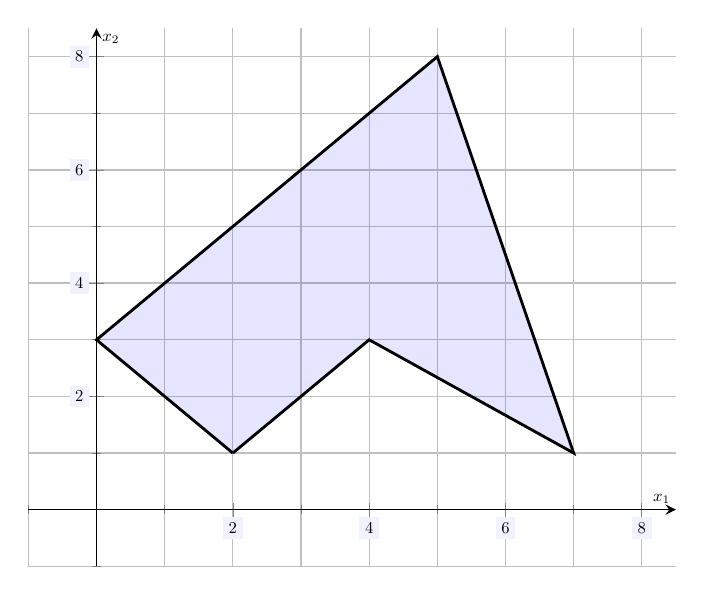
\begin{tikzpicture}[scale=1.2,every node/.style={scale=0.5}]
	\begin{axis}[
	grid=both,
	axis lines=middle,
	ticklabel style={fill=blue!5!white},
	xmin= -1, xmax=8.5,
	ymin= -1, ymax=8.5,
	xtick={0,2,4,6,8},
	ytick={0,2,4,6,8},
	minor tick = {-1,0,1,...,8},
	xlabel=\(x_1\),ylabel=\(x_2\),
	]
	\draw[line width=0.01cm,fill= blue,opacity=0.1] (2,1) -- (0,3) -- (5,8) -- (7,1) -- (4,3) -- (2,1);
	\draw[line width=0.03cm] (2,1) -- (0,3) -- (5,8) -- (7,1) -- (4,3) -- (2,1);
	\end{axis}
	\end{tikzpicture}
	}
	\] \par
Find the maximum and minimum values of $f(x_1, x_2)$ on the region above---if they exist. Be sure to fully justify your answer. 




% Question 9
\newpage
\question[10] Find the initial simplex tableau corresponding to the maximization problem shown below. 
	\[
	\begin{gathered}
	\max z= 2.1x_1 + 6.8x_2 - 4.9x_3 \\
	1.1x_1 + 4.8x_2 - 9.0x_3 \leq 17.5 \\
	2.8x_1 + 15.8x_3 \leq 19.4 \\
	7.4x_1 - 5.6x_2 + 6.8x_3 \geq -18.7 \\
	3.1x_1 + 8.8x_2 - 3.1x_3 \geq 14.9 \\
	x_1, x_2, x_3 \geq 0 
	\end{gathered}
	\]



% Question 10
\newpage
\question[10] Below is the initial simplex tableau corresponding to some maximization problem. Find the corresponding maximization problem. \par
	\begin{table}[!ht]
	\centering
	\begin{tabular}{rrrrrrrrr}
	$3$ & $-1$ & $2$ & $-1$ & $1$ & $0$ & $0$ & $0$ & $22$ \\
	$1$ & $0$ & $6$ & $9$ & $0$ & $1$ & $0$ & $0$ & $15$ \\
	$-2$ & $1$ & $1$ & $-1$ & $0$ & $0$ & $-1$ & $0$ & $4$ \\
	$1$ & $1$ & $1$& $3$ & $0$ & $0$& $0$ & $1$ & $16$ \\
	$-4$ & $3$ & $-5$ & $1$ & $0$ & $0$ & $0$ & $0$ & $0$
	\end{tabular}
	\end{table}



% Question 11
\newpage
\question[10] Below is the final simplex tableau corresponding to some maximization problem. Find the solution to the original optimization problem. \par
	\begin{table}[!ht]
	\centering
	\begin{tabular}{rrrrrrrrr}
	$0$ & $0$ & $1$ & $0.77$ & $0.13$ & $-0.04$ & $0.04$ & $0$ & $16.21$ \\
	$0$ & $1$ & $0$ & $1.34$ & $0.14$ & $0.05$ & $-0.01$ & $0$ & $22.78$ \\
	$1$ & $0$ & $0$ & $1.78$ & $0.06$ & $0.07$ & $0.08$ & $0$ & $45.55$ \\
	$0$ & $0$ & $0$ & $-7.69$ & $-0.2$ & $-0.79$ & $-0.66$ & $1$ & $24.34$ \\
	$0$ & $0$ & $0$ & $12.58$ & $0.49$ & $0.04$ & $0.55$ & $0$ & $220.34$ 	
	\end{tabular}
	\end{table}



% Question 12
\newpage
\question[10] Find the dual problem to the minimization problem shown below. 
	\[
	\begin{gathered}
	\min z= 3x_1 + x_2 + 5x_3 \\
	x_1 + x_2 - x_3 \geq 9 \\
	2x_1 - 5x_2 + x_3 \geq 11 \\
	x_1 - x_3 \geq 6 \\
	x_2 + x_3 \geq 3 \\
	x_1, x_2, x_3 \geq 0 
	\end{gathered}
	\]


\end{questions}
\end{document}